\documentclass{article}

\usepackage[dutch]{babel}
\usepackage{multicol}
\setlength{\columnsep}{1cm}

\usepackage[a4paper,top=2cm,bottom=2cm,left=2cm,right=2cm,marginparwidth=1.75cm]{geometry}

\usepackage{amsmath}
\usepackage{siunitx}
\usepackage{wrapfig}
\usepackage{float}
\usepackage{graphicx}
\usepackage{subcaption}
\usepackage[colorlinks=true, allcolors=blue]{hyperref}
\usepackage{xcolor}
\usepackage{lipsum}
\usepackage{mathtools}
\usepackage{listings}
\usepackage{xcolor}
\usepackage{pdfpages}




\title{Aandrijftechniek maan casus}

\author{Jelmer Hemstra, 1810225, Flint Wardenaar, 1771881}


\begin{document}
\maketitle

\begin{abstract}
    In dit document wordt de casus van de aandrijftechniek van de maanlander behandeld. Hierbij wordt gekeken naar de verschillende aandrijftechnieken en de voor- en nadelen van deze technieken.
\end{abstract}


\section{Inleiding}
    In dit document wordt de casus van de aandrijftechniek van de maanlander behandeld. 


\section{Onderzoek}


    Om te bepalen welk type motor het beste is voor de toepassing wordt er vooral gekeken naar de last die de motor moet verdragen.
    De last is opgedeelt in statische en dynamische last. 
    De statische last is de last die de motor moet verdragen als de maanlander een vaste snelheid heeft.
    De dynamische last is de last die de motor moet verdragen als de maanlander versnelt of vertraagt.
    \newline
    Beschrijf de aanpak en methoden die gebruikt zijn voor het onderzoek en de evaluatie van de motoren en transmissiesystemen.
    Duidelijke formulering van de vraag waarop
    door middel van analyse/onderzoek een
    antwoord wordt gezocht. (max 6 A4’tjes)




\subsection{Analyse van de Last}
    Om de last die de motor moet kunnen verdragen te bepalen wordt er gekeken naar de eisen die aan de maanlander worden gesteld.
    Uit de opdracht die ons gegeven is hebben we de volgende eisen opgesteld:\newline
    - De maanlander moet kunnen rijden op een helling van $20^{\circ}$. \newline
    - de maanlander moet versnellen met $0.7[m/s]$ en vertragen met $0.5[m/s]$. \newline
    - De maanlander moet een top snelheid kunnen halen van $2.1[m/s]$. \newline

    Ook hebben we uit de opdracht de volgende gegevens gehaald:\newline
    - De maanlander heeft een massa van $6[kg]$. \newline
    - De zwaartekracht op de maan is $1.62[m/s^2]$. \newline
    - De rolweerstandscoëfficiënt is $0.1$. \newline
    - De straal van de wielen is $0.075[m]$. \newline
    - De massatraagheid van de wielen is $0.0021[kg \cdot m^2]$. \newline

    Deze last is op te delen in een statische en dynamische last.
    De statische last is de last die de motor moet verdragen als de maanlander een vaste snelheid heeft.
    De dynamische last is de last die de motor moet verdragen als de maanlander versnelt of vertraagt.

\subsubsection{Statische last}
    Er zijn twee onderdelen in de statische last namenlijk de zwaartekracht en de rolweerstand.
    De zwaartekracht is te berekenen met de formule:
    $$F_{zwaartekracht} = m \cdot g \cdot sin(\theta)$$
    - $F_{zwaartekracht}$ is last die de zwaartekracht veroorzaakt in $[N]$ \newline
    - $m$ is de massa van de maanlander in $[kg]$ \newline
    - $g$ is de zwaartekracht in $[m/s^2]$ \newline
    - $\theta$ is de hoek van de helling in $[rad]$ \newline \newline

    De rolweerstand is te berekenen met de formule:
    $$F_{rolweerstand} =  u_{r} \cdot m \cdot g \cdot cos(theta) $$
    - $F_{rolweerstand}$ is de last die de rolweerstand veroorzaakt in $[N]$ \newline
    - $u_{r}$ is de rolweerstandscoëfficiënt \newline
    - $m$ is de massa van de maanlander in $[kg]$ \newline
    - $g$ is de zwaartekracht in $[m/s^2]$ \newline
    - $\theta$ is de hoek van de helling in $[rad]$ \newline \newline

    De totale statische last is dan de som van de zwaartekracht en de rolweerstand:
    $$F_{statisch}[N] = F_{zwaartekracht}[N] + F_{rolweerstand}[N]$$
    Maar om de motor te selecteren moet er gekeken worden naar de koppel. 
    Om de koppel te berekenen per motor moet de volgende formule gebruikt worden:
    $$T_{statisch per wiel}[Nm] = \frac{F_{statisch}[N] \cdot r_{wiel}[m]}{4} $$


\subsubsection{Dynamische last}
    De dynamische last is de last die de motor moet verdragen als de maanlander versnelt of vertraagt. 
    Deze last bestaat uit twee onderdelen: de massatraagheid van de maanlander en de massatraagheid van de wielen.
    De massatraagheid van de maanlander is te berekenen met de formule:
    $$T_{inertiamaanlander} = m \cdot a \cdot r_{wiel}$$
    - $T_{inertiamaanlander}$ is koppel die het kost om de maanlander te versnellen $[Nm]$ \newline
    - $m$ is de massa van de maanlander in $[kg]$ \newline
    - $a$ is de versnelling van de maanlander in $[m/s^2]$ \newline
    - $r_{wiel}$ is de straal van het wiel in $[m]$ \newline \newline

    De massatraagheid van de wielen is te berekenen met de formule:
    $$T_{inertiawielen} = \frac{I_{wielen} \cdot a}{r_{wiel}}$$
    - $T_{inertiawielen}$ is de koppel die het kost om het wiel te versnellen $[Nm]$ \newline
    - $I_{wielen}$ is het traagheidsmoment van de wielen in $[kg \cdot m^2]$ \newline
    - $a$ is de versnelling van de maanlander in $[m/s^2]$ \newline
    - $r_{wiel}$ is de straal van het wiel in $[m]$ \newline \newline

    De totale dynamische koppel per wiel is dan de som van de massatraagheid van de maanlander en de massatraagheid van de wielen:
    $$T_{dynamisch per wiel}[Nm] = \frac{T_{inertiamaanlander}[Nm]}{4} + T_{inertiawielen}[Nm] + T_{statischperwiel}[Nm]$$ 


\subsection{Analyse van de motoren}
\subsubsection{gearbox?}

\section{Resultaten}
    Uitkomsten van de analyse, het onderzoek worden gepresenteerd. max 2 A4tjes

    \subsection{last}
    De statische en dynamische lasten zijn berekend voor verschillende hellingen. 
    Uit deze berekeningen zijn de volgende resultaten gekomen: 

        \begin{table}[h]
            \centering
            \begin{tabular}{|c|c|c|c|c|c|}
            \hline
            Helling & $-20 ^\circ$ & $-8.5 ^\circ$ & $0 ^\circ$ & $8.5 ^\circ$ & $20 ^\circ$ \\ \hline
            Statisch [mNm]  & -45.20   & -8.91   & 18.22   & 44.96  & 79.45   \\ \hline
            Dynamisch [mNm]  & 53.13  & 89.43   & 116.57  & 143.31  & 177.81  \\ \hline
            \end{tabular}
            \caption{Helling - Koppel}
            \label{tab}
        \end{table}
        Dit is gedaan met de volgende formules:
        $$T_{statisch} = \frac{r_{wiel}(m \cdot g \cdot sin(\theta) + u_r \cdot m \cdot g \cdot cos(\theta))}{4} = \frac{0.075(9.72 \cdot sin(\theta) +  0.972 \cdot cos(\theta))}{4}$$
        $$T_{dynamisch} = T_{statisch} + \frac{m \cdot a \cdot r_{wiel}}{4} + \frac{I_{wielen} \cdot a}{r_{wiel}} = T_{statisch} + \frac{0.315}{4}+ 0.0196 $$
        Deze formules zijn toegelicht in hoofdstuk 2.1.
        
    \subsection{Motor}
    De motor is gekozen aan de hand van de tabel in 3.1. 
    Ook is er gekeken naar de gearbox daar geldt namenlijk dat hoe minder vertanding de gearbox hoeft te doen hoe efficienter deze is. 
    Hierdoor is er gekozen voor een so traag mogelijke motor binnen de RE25 1187 serie.
    De motor die gekozen is is de RE25 118745. 
    Deze motor heeft een No-load speed van 4790 [rpm], een maximale efficientie van 90 procent en een nominale koppel van 28.7 [mNm].
    De nominale snelheid van de motor is 3710 [rpm].
    

    \subsection{gearhead}
    De gearbox is gekozen aan de hand van de motor. 
    In de datasheet van de motor worden namenlijk een aantal gearboxes aangeraden.
    Een daarvan is degende die wij gekozen hebben, namenlijk de GP 26A 406757. 
    Deze gearbox heeft een vertanding van 5.2:1. dit zorgt voor een Nominale snelheid van 710 [rpm] en een nominale koppel van 150 [mNm]. 
    Dit is meer dan genoeg koppel om met een constante snelheid van 2.1 [m/s] te rijden op een helling van 20 graden.

\section{Advies}
    De


% All other content before appendices should go above this line
% Now, include the PDF files as appendices
% Place this right before the appendix command
\clearpage
\appendix
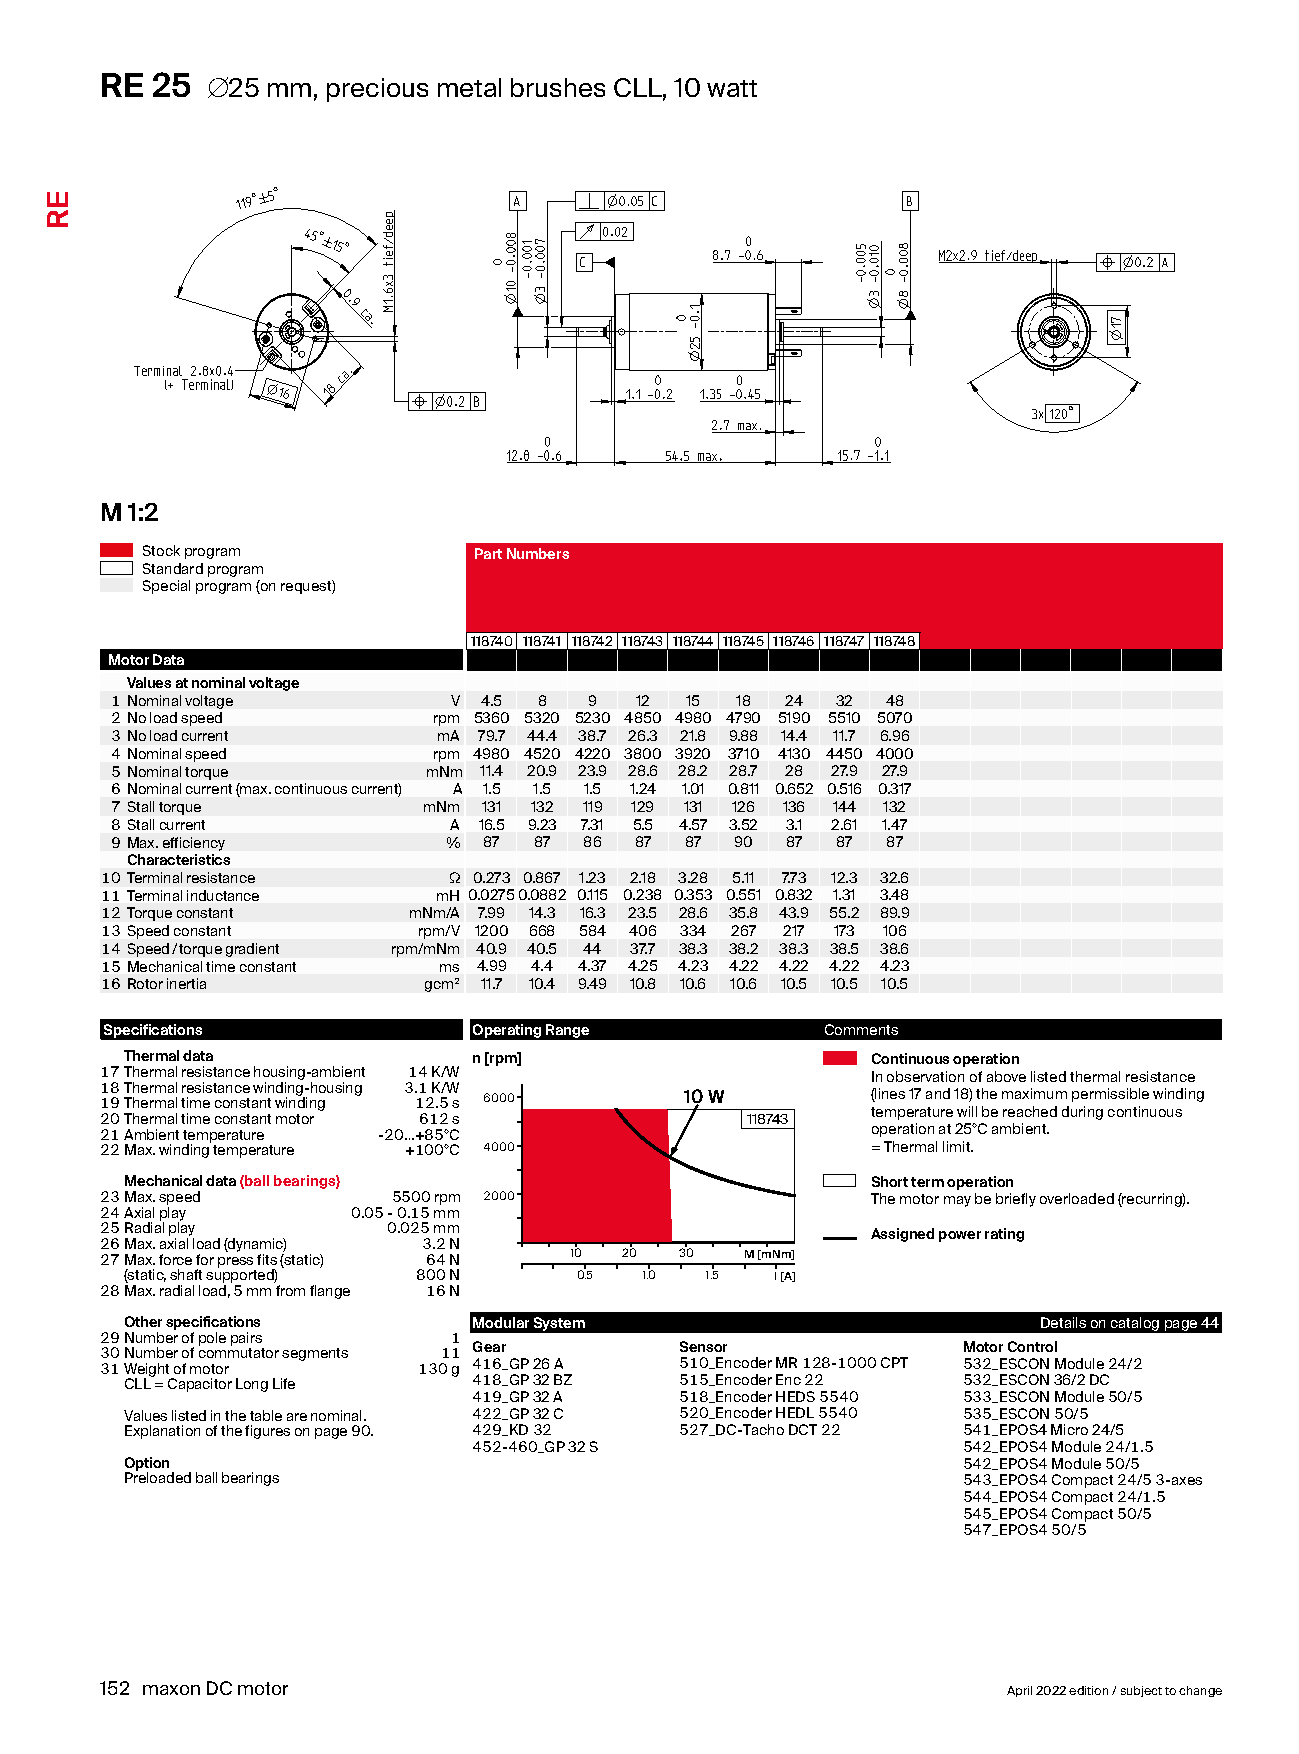
\includepdf[pages=-]{EN-22-152.pdf}
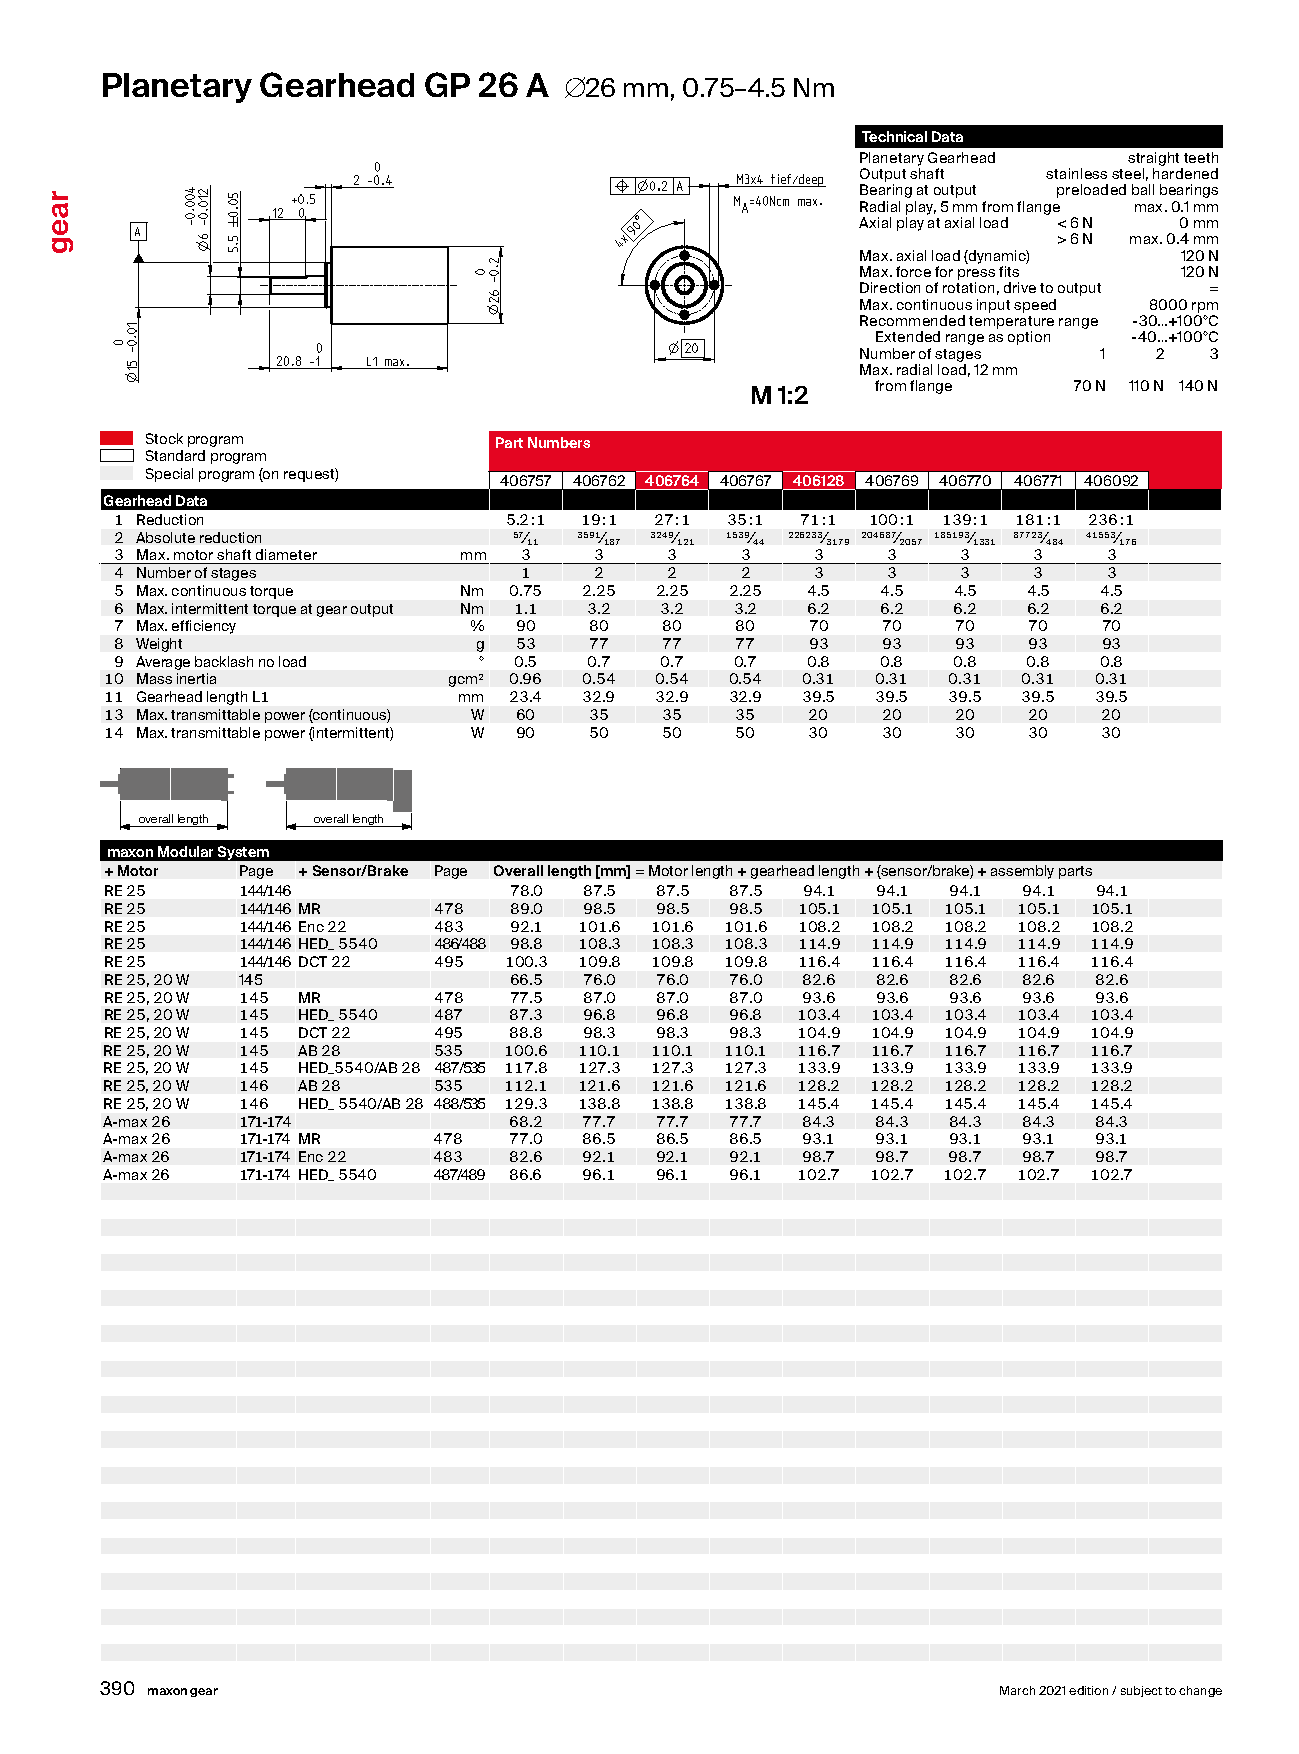
\includepdf[pages=-]{EN-21-390.pdf}

\end{document}